\documentclass[a4paper,14pt]{extarticle}

\usepackage[a4paper,top=20mm,bottom=20mm,left=30mm,right=10mm]{geometry}
\usepackage[T1,T2A]{fontenc}
\usepackage[utf8]{inputenc}
\usepackage[russian]{babel}
\usepackage{indentfirst}
\usepackage{titlesec}
\usepackage{graphicx}
\usepackage{listings}

\renewcommand{\baselinestretch}{1.3}
\titleformat{\section}{\normalsize\bfseries}{\thesection}{1em}{}
\titleformat{\subsection}{\normalsize\bfseries}{\thesection}{1em}{}
\setlength{\parindent}{12.5mm}

\begin{document}
	
	\newpage\thispagestyle{empty}
	\begin{center}
		\MakeUppercase{
			Министерство науки и высшего образования Российской Федерации\\
			Федеральное государственное бюджетное образовательное учреждение высшего образования\\
			<<Вятский Государственный Университет>>\\
		}
		Институт математики и информационных систем\\
		Факультет автоматики и вычислительной техники\\
		Кафедра электронных вычислительных машин
	\end{center}
	\vfill
	
	\begin{center}
		Отчет по лабораторной работе №6\\
		по дисциплине\\
		<<Информатика>>\\
		<<Кодирование информации>>
	\end{center}
	\vfill
	
	\noindent
	\begin{tabular}{ll}
		Выполнил студент гр. ИВТб-1301-05-00 \hspace{5mm} &
		\rule[-1mm]{25mm}{0.10mm}\,/Макаров С.А./\\
		
		Руководитель доцент кафедры ЭВМ & \rule[-1mm]{25mm}{0.10mm}\,/Коржавина А.С./\\
	\end{tabular}
	
	\vfill
	\begin{center}
		Киров 2024
	\end{center}
	
	\newpage
	\section*{Цель}
	Цель лабораторной работы: закрепить на практике знания кодирования информации. Написать программы, решающие описанные ниже задачи.
	
	\section*{Задание}
	\begin{enumerate}
		\item Равномерное кодирование. Написать программу, выполняющую кодирование N различных состояний равномерно. На входе: целое число N -- количество различных состояний, на выходе -- список кодов.
		
		\item Оптимальное кодирование. Написать программу, выполняющую кодирование алгоритмом Хаффмана или Фано. На входе через пробел: количество событий (кодовых состояний), массив вероятностей каждого из событий. На выходе: коды состояний.
	\end{enumerate}
	
	\newpage
	\section*{Решение}
	\subsection*{Задание 1}
	Схема алгоритма для решения предлагаемой задачи представлена на рисунке 1.
	\begin{figure}[h]
		\centering
		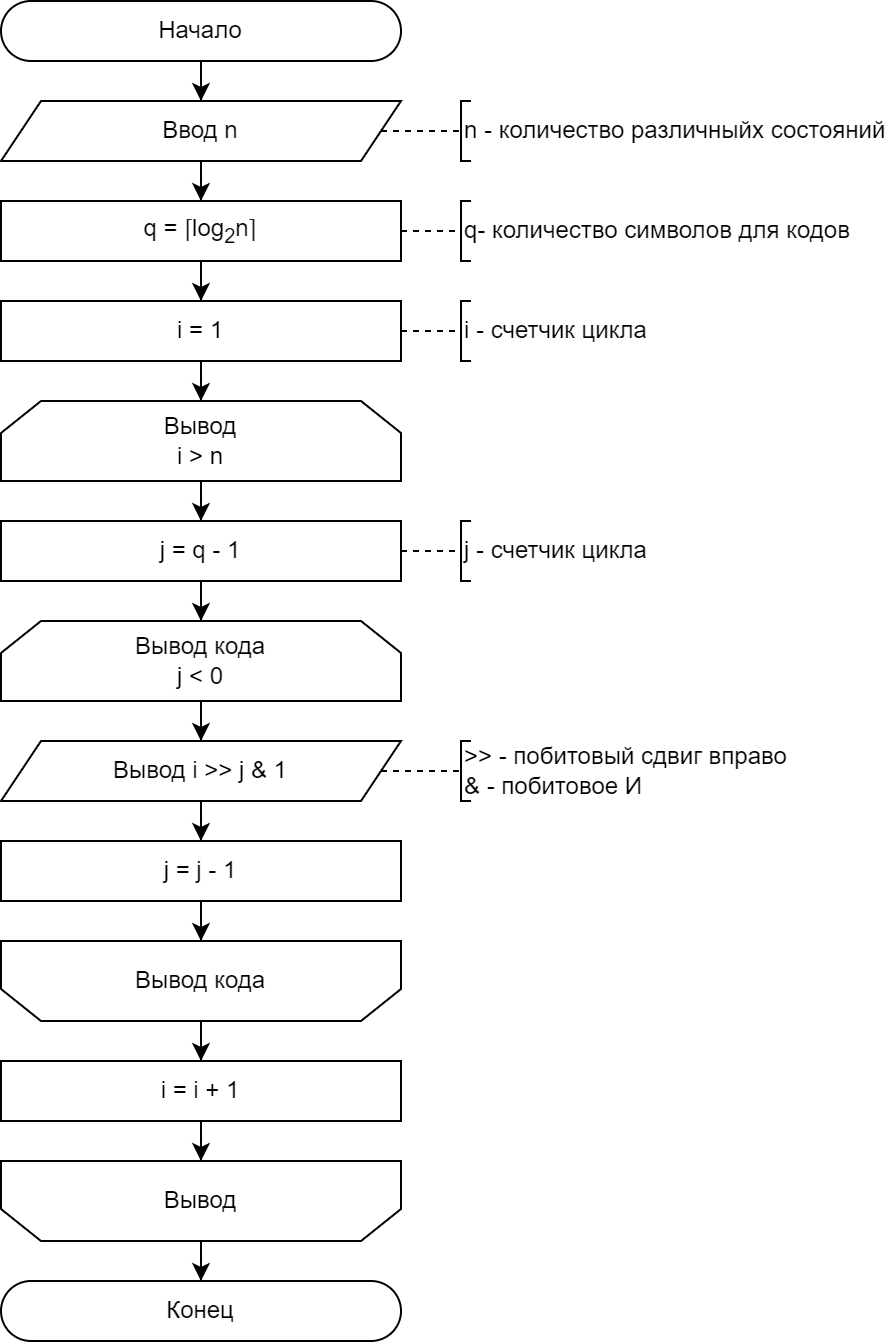
\includegraphics[width=0.6\linewidth]{schemes/s-1}
	\end{figure}
	\begin{center}
		Рисунок 1 – Схема алгоритма задания 1
	\end{center}
	
	\pagebreak
	Решение задачи на языке C представлено ниже.
	\begin{lstlisting}[tabsize=2,basicstyle=\ttfamily]
#include <stdio.h>
#include <math.h>

int main() {
	int n;
	scanf("%d", &n);
	
	int q = ceil(log2(n));
	
	for (int i = 0; i < n; i++) {
		for (int j = q - 1; j >= 0; j--) {
			printf("%d", i >> j & 1);
		}
		printf(" ");
	}
	
	return 0;
}
	\end{lstlisting}
	
	\newpage
	\subsection*{Задание 2}
	Схема алгоритма для решения предлагаемой задачи представлена на рисунках 2.1, 2.2, 2.3.
	
	\begin{figure}[h]
		\centering
		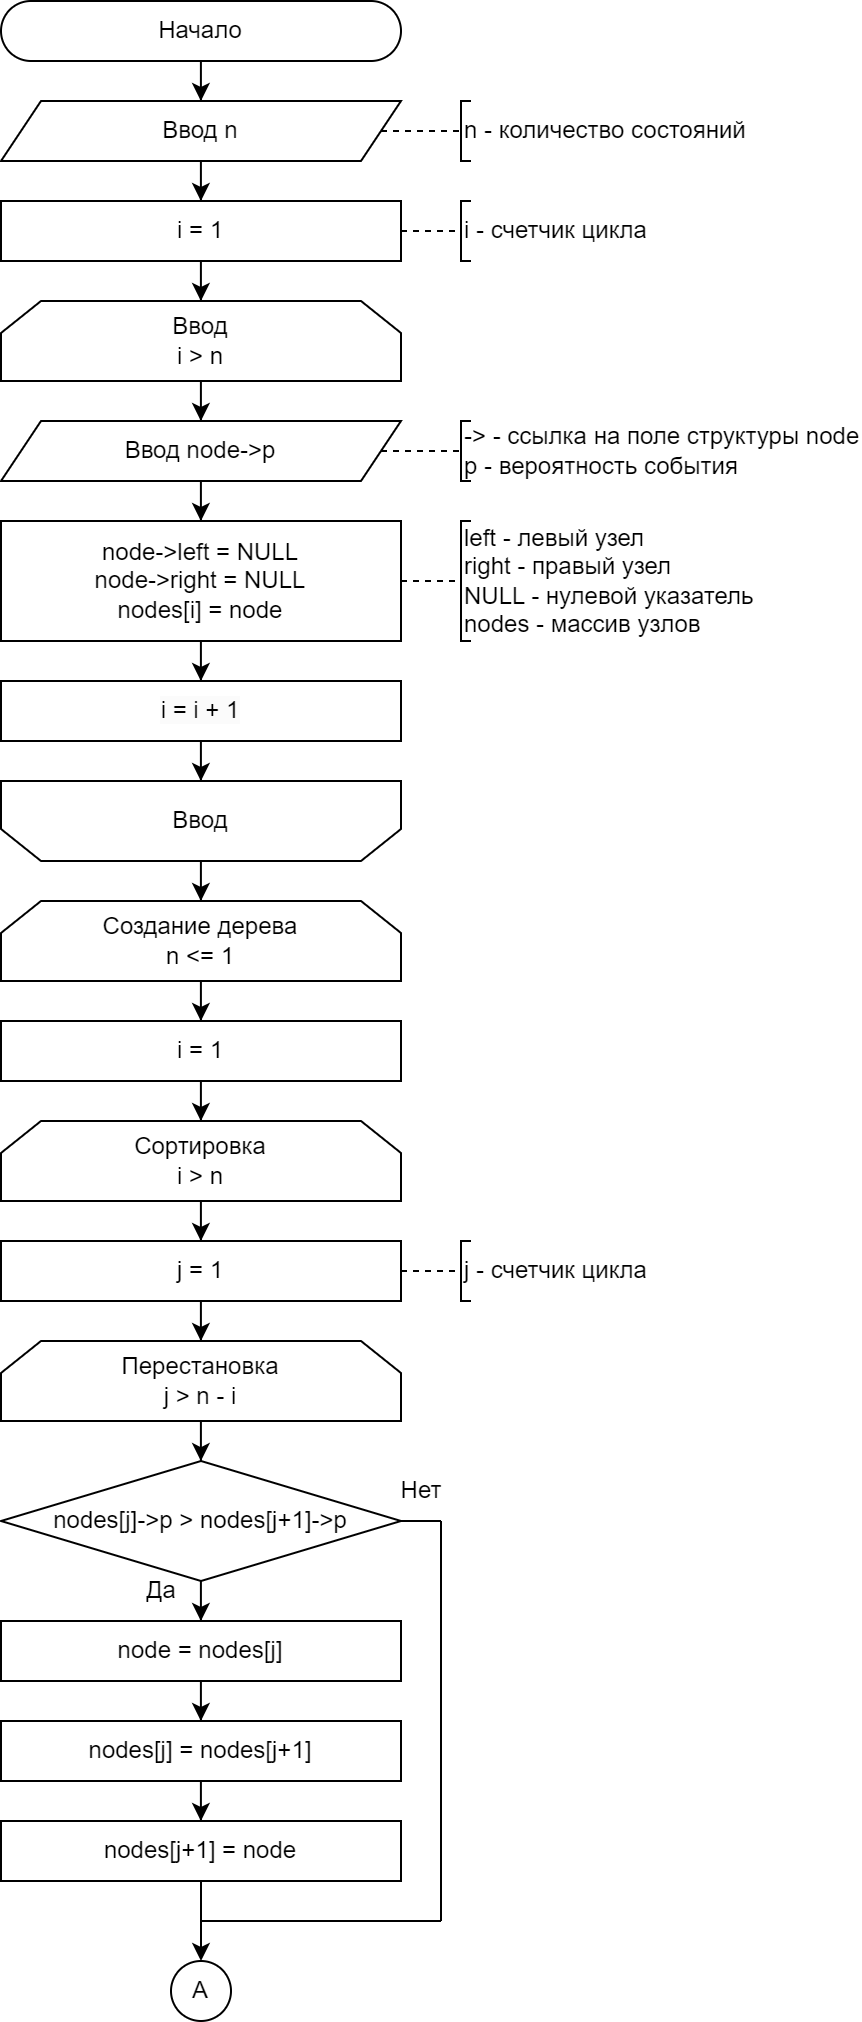
\includegraphics[width=0.5\linewidth]{schemes/s-2-1}
	\end{figure}
	\begin{center}
		Рисунок 2.1 – Схема алгоритма задания 2
	\end{center}
	\pagebreak
	
	\begin{figure}[h]
		\centering
		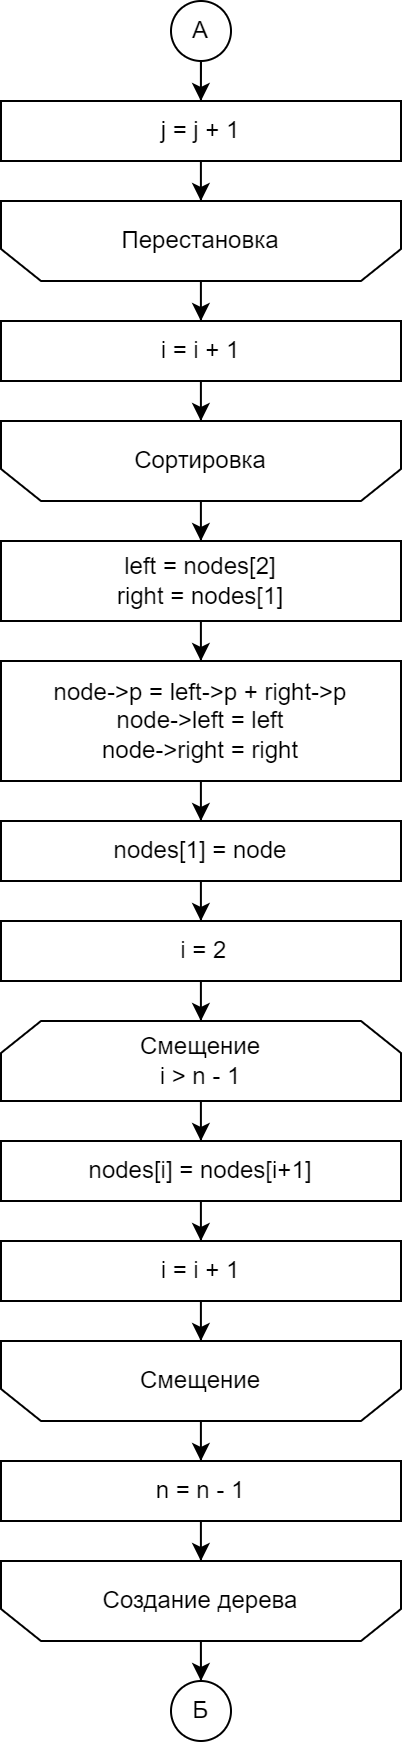
\includegraphics[width=0.27\linewidth]{schemes/s-2-2}
	\end{figure}
	\begin{center}
		Рисунок 2.2 – Продолжение схемы алгоритма задания 2
	\end{center}
	\pagebreak
	
	\begin{figure}[h]
		\centering
		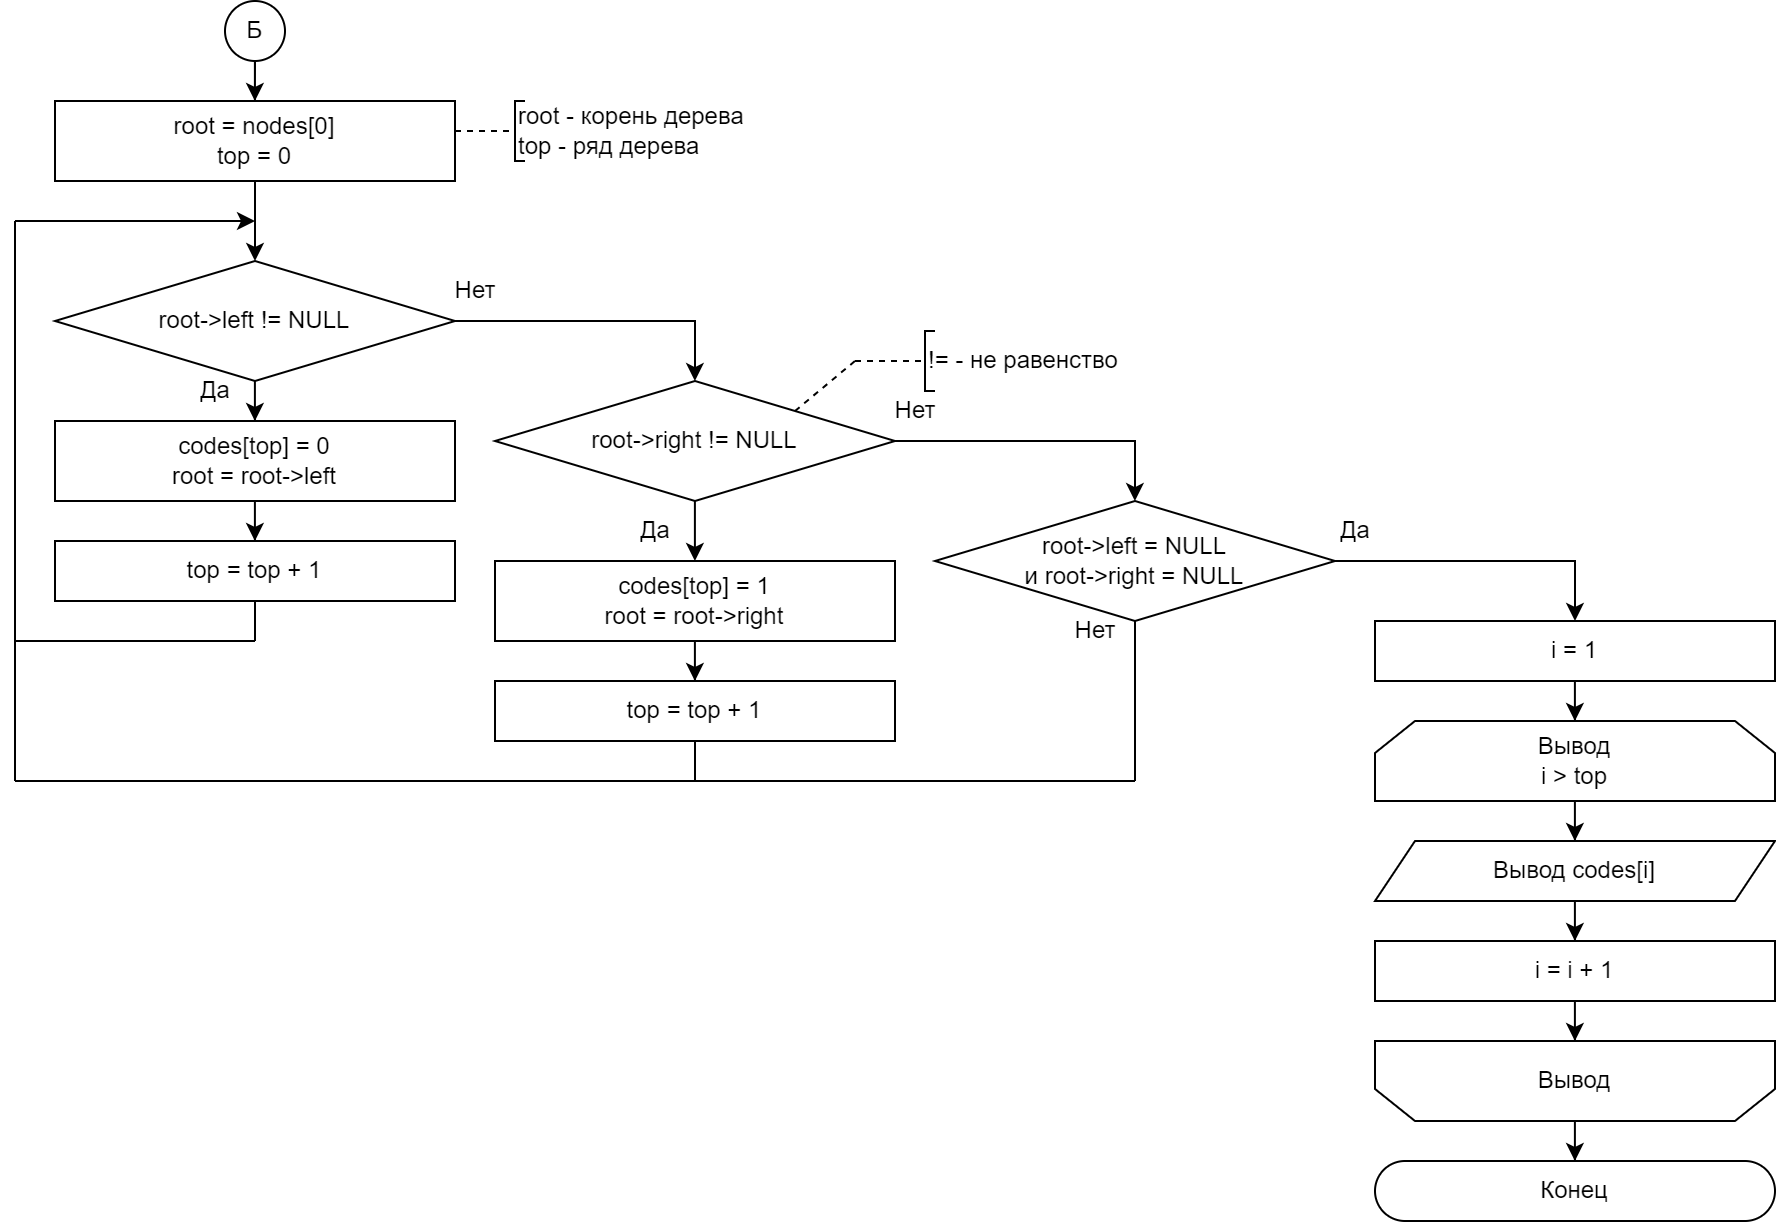
\includegraphics[width=1\linewidth]{schemes/s-2-3}
	\end{figure}
	\begin{center}
		Рисунок 2.3 – Продолжение схемы алгоритма задания 2
	\end{center}
	
	Решение задачи на языке C представлено ниже.
	\begin{lstlisting}[tabsize=2,basicstyle=\ttfamily]
#include <stdio.h>
#include <stdlib.h>

typedef struct Node {
	float p;
	struct Node *left, *right;
} Node;

void print_code(Node* root, int codes[], int top) {
	if (root->left) {
		codes[top] = 0;
		print_code(root->left, codes, top + 1);
	}
	
	if (root->right) {
		codes[top] = 1;
		print_code(root->right, codes, top + 1);
	}
	
	if (root->left == NULL && root->right == NULL) {
		for (int i = 0; i < top; i++) {
			printf("%d", codes[i]);
		}
		printf(" ");
	}
}

int main() {
	int n;
	scanf("%d", &n);
	
	struct Node* nodes[n];
	
	for (int i = 0; i < n; i++) {
		Node* node = (Node*)malloc(sizeof(Node));
		scanf("%f", &node->p);
		node->left = NULL;
		node->right = NULL;
		nodes[i] = node;
	}
	
	
	while (n > 1) {
		for (int i = 0; i < n - 1; i++) {
			for (int j = 0; j < n - i - 1; j++) {
				if (nodes[j]->p > nodes[j + 1]->p) {
					Node* node = nodes[j];
					nodes[j] = nodes[j + 1];
					nodes[j + 1] = node;
				}
			}
		}
		
		Node* left = nodes[1];
		Node* right = nodes[0];
		Node* node = (Node*)malloc(sizeof(Node));
		node->p = left->p + right->p;
		node->left = left;
		node->right = right;
		nodes[0] = node;
		
		for (int i = 1; i < n - 1; i++) {
			nodes[i] = nodes[i + 1];
		}
		
		n--;
	}
	
	int codes[32];
	print_code(nodes[0], codes, 0);
	
	return 0;
}
	\end{lstlisting}

	\section*{Вывод}
	В ходе лабораторной работы удалось закрепить на практике знания равномерного и оптимального кодирования, реализовав программы, формирующие равномерный код и оптимальный код с учетом вероятности того или иного события.
	
\end{document}